% -----------------------------*- LaTeX -*------------------------------
\documentclass[UTF8]{article}
% ------------------------------------------------------------------------
% Packages
% ------------------------------------------------------------------------
\usepackage{ctex} % 支持中文
\usepackage[body={7in, 9in},left=1in,right=1in]{geometry} % 改变页边距
\usepackage{amsmath} % AMS 的数学宏包
\usepackage{amsfonts} % AMS 的数学字体宏包
\usepackage{amssymb} % AMS 符号库
\usepackage{bm} % 数学公式中的黑斜体
\usepackage{amsthm} % AMS 的定理环境宏包
\usepackage{graphicx} % 插图
\usepackage{subfigure} % 插子图
\usepackage{nicefrac} % 好看的分数
\usepackage{mathrsfs} % mathscr font
\usepackage{caption} % caption
\usepackage{algorithm,algorithmicx} % 伪代码支持宏包
\usepackage[noend]{algpseudocode} % 伪代码
\usepackage{fancyhdr} % 设置页眉、页脚
\usepackage{adjustbox} % 图片尺寸自动调整
\usepackage{esint} % 积分符号
\usepackage{mathtools} % 数学宏包的重要补充
\usepackage{upgreek} % 数学环境的直立希腊字母
\usepackage{enumitem} % 使用enumitem宏包, 改变列表项的格式
\usepackage{color} % 支持彩色
\usepackage{extarrows} % 任意长度的箭头
\usepackage{tikz} % 绘图
\usepackage{forest} % 绘树
\usepackage{xcolor} % 颜色宏包
\usepackage{breqn} % 公式自动换行
\usepackage{fontsize} % 字体大小
\usepackage[framemethod=TikZ]{mdframed} % 给文字加框
\usepackage{fontspec} % 字体库
\usepackage{bigstrut} % 用于表格中的换行
\usepackage{multirow} % 表格中多行单元格合并
\usepackage{multicol} % 表格中多列单元格合并
\usepackage{longtable} % 长表格
\usepackage{rotating} % 旋转图形和表格      以上三者用于绘制三线表
\usepackage{booktabs} % 三线表宏包
\usepackage{scribe} % Scribe 模板
\usepackage{diagbox} % 表格斜线
\usepackage{listings} % 插入代码
\usetikzlibrary{automata} % 引入automata库
\usetikzlibrary{shapes,arrows,positioning,chains} % 引入positioning库
% ------------------------------------------------------------------------
% Macros
% ------------------------------------------------------------------------
%~~~~~~~~~~~~~~~
% Utility latin
%~~~~~~~~~~~~~~~
\newcommand{\ie}{\textit{i.e.}}
\newcommand{\eg}{\textit{e.g.}}
%~~~~~~~~~~~~~~~
% Environment shortcuts
%~~~~~~~~~~~~~~~
\newcommand{\balign}[1]{\ealign{\begin{align}#1\end{align}}}
\newcommand{\baligns}[1]{\ealigns{\begin{align*}#1\end{align*}}}
\newcommand{\bitemize}[1]{\eitemize{\begin{itemize}#1\end{itemize}}}
\newcommand{\benumerate}[1]{\eenumerate{\begin{enumerate}#1\end{enumerate}}}
%~~~~~~~~~~~~~~~
% Text with quads around it
%~~~~~~~~~~~~~~~
\newcommand{\qtext}[1]{\quad\text{#1}\quad}
%~~~~~~~~~~~~~~~
% Shorthand for math formatting
%~~~~~~~~~~~~~~~
\newcommand{\mbb}[1]{\mathbb{#1}}
\newcommand{\mbi}[1]{\boldsymbol{#1}} % Bold and italic (math bold italic)
\newcommand{\mbf}[1]{\mathbf{#1}}
\newcommand{\mc}[1]{\mathcal{#1}}
\newcommand{\mrm}[1]{\mathrm{#1}}
\newcommand{\tbf}[1]{\textbf{#1}}
\newcommand{\tsc}[1]{\textsc{#1}}
%\def\\langle {{\langle }}
%\def\\rangle {{\rangle }}
\newcommand{\sT}{\sf T}
\newcommand{\grad}{\nabla}
\newcommand{\Proj}{\Pi}
%~~~~~~~~~~~~~~~
% Common sets 定义数集符号
%~~~~~~~~~~~~~~~
\newcommand{\R}{\mathbb{R}}
\newcommand{\Z}{\mathbb{Z}}
\newcommand{\Q}{\mathbb{Q}}
\newcommand{\N}{\mathbb{N}}
\newcommand{\C}{\mathbb{C}}
\newcommand{\reals}{\mathbb{R}} % Real number symbol
\newcommand{\integers}{\mathbb{Z}} % Integer symbol
\newcommand{\rationals}{\mathbb{Q}} % Rational numbers
\newcommand{\naturals}{\mathbb{N}} % Natural numbers
\newcommand{\complex}{\mathbb{C}} % Complex numbers
%~~~~~~~~~~~~~~~
% Common functions
%~~~~~~~~~~~~~~~
\renewcommand{\exp}[1]{\operatorname{exp}\left(#1\right)} % Exponential
\newcommand{\indic}[1]{\mbb{I}\left(#1\right)} % Indicator function
\newcommand{\indicsub}[2]{\mbb{I}_{#2}\left(#1\right)} % Indicator function
\newcommand{\argmax}{\mathop\mathrm{arg\, max}} % Defining math symbols
\newcommand{\argmin}{\mathop\mathrm{arg\, min}}
\renewcommand{\arccos}{\mathop\mathrm{arccos}}
\newcommand{\dom}{\mathop\mathrm{dom}} % Domain
\newcommand{\range}{\mathop\mathrm{range}} % Range
\newcommand{\diag}{\mathop\mathrm{diag}}
\newcommand{\tr}{\mathop\mathrm{tr}}
\newcommand{\abs}{\mathop\mathrm{abs}}
\newcommand{\card}{\mathop\mathrm{card}}
\newcommand{\sign}{\mathop\mathrm{sign}}
\newcommand{\prox}{\mathrm{prox}} % prox
\newcommand{\rank}[1]{\mathrm{rank}(#1)}
\newcommand{\supp}[1]{\mathrm{supp}(#1)}
\newcommand{\norm}[1]{\lVert#1\rVert}
%~~~~~~~~~~~~~~~
% Common probability symbols
%~~~~~~~~~~~~~~~
\newcommand{\family}{\mathcal{P}} % probability family / statistical model
\newcommand{\iid}{\stackrel{\mathrm{iid}}{\sim}}
\newcommand{\ind}{\stackrel{\mathrm{ind}}{\sim}}
\newcommand{\E}{\mathbb{E}} % Expectation symbol
\newcommand{\Earg}[1]{\E\left[#1\right]}
\newcommand{\Esubarg}[2]{\E_{#1}\left[#2\right]}
\renewcommand{\P}{\mathbb{P}} % Probability symbol
\newcommand{\Parg}[1]{\P\left(#1\right)}
\newcommand{\Psubarg}[2]{\P_{#1}\left[#2\right]}
%\newcommand{\Cov}{\mrm{Cov}} % Covariance symbol
%\newcommand{\Covarg}[1]{\Cov\left[#1\right]}
%\newcommand{\Covsubarg}[2]{\Cov_{#1}\left[#2\right]}
%\newcommand{\model}{\mathcal{P}} % probability family / statistical model
%~~~~~~~~~~~~~~~
% Distributions
%~~~~~~~~~~~~~~~
%\newcommand{\Gsn}{\mathcal{N}}
%\newcommand{\Ber}{\textnormal{Ber}}
%\newcommand{\Bin}{\textnormal{Bin}}
%\newcommand{\Unif}{\textnormal{Unif}}
%\newcommand{\Mult}{\textnormal{Mult}}
%\newcommand{\NegMult}{\textnormal{NegMult}}
%\newcommand{\Dir}{\textnormal{Dir}}
%\newcommand{\Bet}{\textnormal{Beta}}
%\newcommand{\Gam}{\textnormal{Gamma}}
%\newcommand{\Poi}{\textnormal{Poi}}
%\newcommand{\HypGeo}{\textnormal{HypGeo}}
%\newcommand{\GEM}{\textnormal{GEM}}
%\newcommand{\BP}{\textnormal{BP}}
%\newcommand{\DP}{\textnormal{DP}}
%\newcommand{\BeP}{\textnormal{BeP}}
%\newcommand{\Exp}{\textnormal{Exp}}
%~~~~~~~~~~~~~~~
% Theorem-like environments
%~~~~~~~~~~~~~~~
%\theoremstyle{definition}
%\newtheorem{definition}{Definition}
%\newtheorem{example}{Example}
%\newtheorem{problem}{Problem}
%\newtheorem{lemma}{Lemma}
%~~~~~~~~~~~~~~~
% 组合数学的模板和作业里用到的一些宏包和自定义命令
%~~~~~~~~~~~~~~~
\renewcommand{\emph}[1]{\begin{kaishu}#1\end{kaishu}}
\newcommand{\falfac}[1]{^{\underline{#1}}}
\newcommand{\binomfrac}[2]{\frac{#1^{\underline{#2}}}{#2!}}
\newcommand{\ceil}[1]{\left\lceil #1 \right\rceil}
\newcommand{\floor}[1]{\left\lfloor #1 \right\rfloor}
\newcommand{\suminfty}[2]{\sum_{#1=#2}^{\infty}}
\newcommand{\suminftyk}[0]{\sum_{k=0}^{\infty}}
\newcommand{\sumint}[3]{\sum_{#1=#2}^{#3}}
\newcommand{\sumintk}[2]{\sum_{k=#1}^{#2}}
\newcommand{\suminti}[2]{\sum_{i=#1}^{#2}}
%~~~~~~~~~~~~~~~
% 定义新命令
%~~~~~~~~~~~~~~~
\newcommand*{\unit}[1]{\mathop{}\!\mathrm{#1}}
\newcommand*{\dif}{\mathop{}\!\mathrm{d}}%微分算子 d
\newcommand*{\pdif}{\mathop{}\!\partial}%偏微分算子
\newcommand*{\cdif}{\mathop{}\!\nabla}%协变导数、nabla 算子
\newcommand*{\laplace}{\mathop{}\!\Delta}%laplace 算子
\newcommand*{\deri}[1]{\mathrm{d} #1}
\newcommand*{\deriv}[2]{\frac{\mathrm{d} #1}{\mathrm{d} {#2}}}
\newcommand*{\derivh}[3]{\frac{\mathrm{d}^{#1} #2}{\mathrm{d} {#3^{#1}}}}
\newcommand*{\pderiv}[2]{\frac{\partial #1}{\partial {#2}}}
\newcommand*{\pderivh}[3]{\frac{\partial^{#1} #2}{\partial {#3^{#1}}}}
\newcommand*{\dderiv}[2]{\dfrac{\mathrm{d} #1}{\mathrm{d} {#2}}}
\newcommand*{\dderivh}[3]{\dfrac{\mathrm{d}^{#1} #2}{\mathrm{d} {#3^{#1}}}}
\newcommand*{\dpderiv}[2]{\dfrac{\partial #1}{\partial {#2}}}
\newcommand*{\dpderivh}[3]{\dfrac{\partial^{#1} #2}{\partial {#3^{#1}}}}
\newcommand{\me}[1]{\mathrm{e}^{#1}}%e 指数
\newcommand{\mi}{\mathrm{i}}%虚数单位
%\newcommand{\mc}{\mathrm{c}}%光速 定义与mathcal冲突
\newcommand{\red}[1]{\textcolor{red}{#1}}
\newcommand{\blue}[1]{\textcolor{blue}{#1}}
%\newcommand{\Rome}[1]{\setcounter{rome}{#1}\Roman{rome}}
%~~~~~~~~~~~~~~~
% 公式环境中箭头符号的简写
%~~~~~~~~~~~~~~~
\newcommand{\ra}{\rightarrow}
\newcommand{\Ra}{\Rightarrow}
\newcommand{\la}{\leftarrow}
\newcommand{\La}{\Leftarrow}
\newcommand{\lra}{\leftrightarrow}
\newcommand{\Lra}{\Leftrightarrow}
\newcommand{\lgla}{\longleftarrow}
\newcommand{\Lgla}{\Longleftarrow}
\newcommand{\lgra}{\longrightarrow}
\newcommand{\Lgra}{\Longrightarrow}
\newcommand{\lglra}{\longleftrightarrow}
\newcommand{\Lglra}{\Longleftrightarrow}
%~~~~~~~~~~~~~~~
% 一些数学的环境设置
%~~~~~~~~~~~~~~~
%\newcounter{counter_exm}\setcounter{counter_exm}{1}
%\newcounter{counter_prb}\setcounter{counter_prb}{1}
%\newcounter{counter_thm}\setcounter{counter_thm}{1}
%\newcounter{counter_lma}\setcounter{counter_lma}{1}
%\newcounter{counter_dft}\setcounter{counter_dft}{1}
%\newcounter{counter_clm}\setcounter{counter_clm}{1}
%\newcounter{counter_cly}\setcounter{counter_cly}{1}
\newtheorem{theorem}{{\hskip 1.7em \bf 定理}}
\newtheorem{lemma}[theorem]{\hskip 1.7em 引理}
\newtheorem{proposition}[theorem]{\hskip 1.7em 命题}
\newtheorem{claim}[theorem]{\hskip 1.7em 断言}
\newtheorem{corollary}[theorem]{\hskip 1.7em 推论}
% \newcommand{\problem}[1]{{\setlength{\parskip}{10pt}\noindent \bf{#1}}}
\newenvironment{solution}{{\noindent \bf 解 \quad}}{}
\newenvironment{remark}{{\noindent \bf 注 \quad}}{}
\newenvironment{definition}{{\noindent \bf 定义 \quad}}{}
\renewenvironment{proof}{{\setlength{\parskip}{7pt}\noindent\hskip 2em \bf 证明 \quad}}{\hfill$\qed$\par}
\newenvironment{example}{{\noindent\bf 例 \quad}}{\hfill$\qed$\par}
%\newenvironment{concept}[1]{{\bf #1\quad} \begin{kaishu}} {\end{kaishu}\par}
%~~~~~~~~~~~~~~~
% 本.tex文档中特殊定义命令
%~~~~~~~~~~~~~~~
\newcommand{\lno}[1]{\overline{#1}}
\newcommand{\NP}{\mathrm{NP}}
\newcommand{\coNP}{\mathrm{coNP}}
% \newcommand{\ISO}{\mathrm{ISO}}
\newcommand{\SAT}{\mathrm{SAT}}
\newcommand{\USAT}{\mathrm{USAT}}
% \newcommand{\threeSAT}{\mathrm{3\text{-}SAT}}
\renewcommand{\P}{\mathrm{P}}
% \mathchardef\mhyphen="2D
% \newcommand{\CNF}{\mathrm{CNF}}
% \newcommand{\DNF}{\mathrm{DNF}}
% \newcommand{\SetSp}{\mathrm{SET\text{-}SPLITTING}}
% \newcommand{\PUZZLE}{\mathrm{PUZZLE}}
% \newcommand{\SPATH}{\mathrm{SPATH}}
% \newcommand{\LPATH}{\mathrm{LPATH}}
% \newcommand{\UHAMPATH}{\mathrm{UHAMPATH}}
\newcommand{\SPACE}{\mathrm{SPACE}}
\newcommand{\NSPACE}{\mathrm{NSPACE}}
\newcommand{\PSPACE}{\mathrm{PSPACE}}
\newcommand{\NPSPACE}{\mathrm{NPSPACE}}
\newcommand{\DFA}{\mathrm{DFA}}
\newcommand{\NFA}{\mathrm{NFA}}
\newcommand{\TQBF}{\mathrm{TQBF}}
% \newcommand{\L}{\mathrm{L}}
\renewcommand{\O}{\mathrm{O}}
\newcommand{\NL}{\mathrm{NL}}
\newcommand{\coNL}{\mathrm{coNL}}
\newcommand{\LADDER}{\mathrm{LADDER_{DFA}}}
\newcommand{\hd}{\mathrm{\text{-}hard}}
\newcommand{\ADD}{\mathrm{ADD}}
\newcommand{\STCN}{\mathrm{STRONGLY\text{-}CONNECTED}}
\newcommand{\PATH}{\mathrm{PATH}}
\newcommand{\A}{\mathrm{A}}
%使用align环境公式换页
\allowdisplaybreaks[4]

\definecolor{dkgreen}{rgb}{0,0.6,0}
\definecolor{gray}{rgb}{0.5,0.5,0.5}
\definecolor{mauve}{rgb}{0.58,0,0.82}
\lstset{
  frame=tb,
  aboveskip=3mm,
  belowskip=3mm,
  showstringspaces=false,
  columns=flexible,
  framerule=1pt,
  rulecolor=\color{gray!35},
  backgroundcolor=\color{gray!5},
  basicstyle={\small\ttfamily},
  numbers=none,
  numberstyle=\tiny\color{gray},
  keywordstyle=\color{blue},
  commentstyle=\color{dkgreen},
  stringstyle=\color{mauve},
  breaklines=true,
  breakatwhitespace=true,
  tabsize=3,
}

\setmainfont{Times New Roman}
\setsansfont{Times New Roman}
\setmonofont{Consolas}
\setCJKmainfont{SimHei}
\setCJKsansfont{SimSun}
\setCJKmonofont{FangSong}
\punctstyle{kaiming}

\begin{document}

\pagestyle{fancy}
\lhead{\emph{计算机网络实验课}}
\chead{\emph{中国科学院大学}}
\rhead{\emph{2022K800992910张家玮}}

\begin{center}
    {\LARGE \bf 二 \quad Socket应用编程实验}
\end{center}

\section{实验目的}

使用C语言实现最简单的HTTP服务器,使用两个线程分别同时监听支持HTTP(80端口)和HTTPS(443端口)。只需支持GET方法,解析请求报文,返回相应应答及内容。需要支持以下状态码:

\begin{figure}[H]
    \centering
    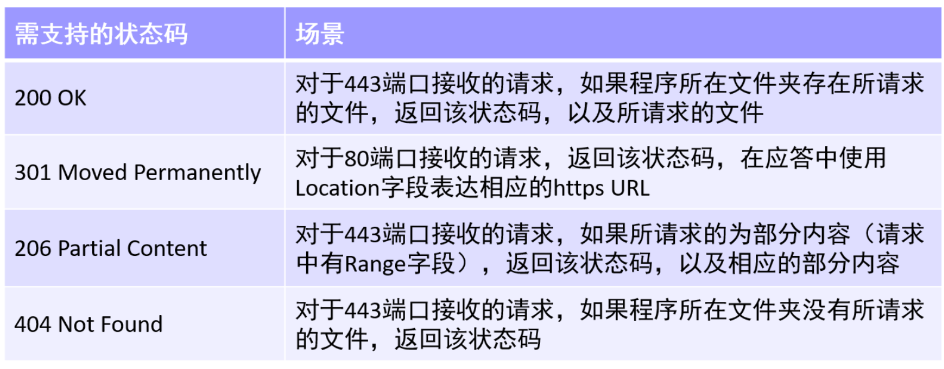
\includegraphics[width=0.8\textwidth]{status_code.png}
    \caption{需要支持的状态码}
\end{figure}

\section{实验流程}

\begin{enumerate}
    \item 根据上述要求,实现HTTP服务器程序;
    \item 执行sudo python topo.py命令,生成包括两个端节点的网络拓扑;
    \item 在主机h1上运行HTTP服务器程序,同时监听80和443端口:
    \begin{lstlisting}[language=bash]
        ./http-server
    \end{lstlisting}
    \item 在主机h2上运行测试程序,验证程序正确性:
    \begin{lstlisting}[language=bash]
        python3 test/test.py # 如果没有出现AssertionError或其他错误,则说明程序实现正确
    \end{lstlisting}
    \item 代码提交到OJ网站,报告提交到课程网站。
\end{enumerate}

\section{实验分析}

在\texttt{main}函数中创建两个线程,分别监听80和443端口:

\begin{lstlisting}[language=c]
int main(){   
    pthread_t http, https;
    if (pthread_create(&http, NULL, HTTP_SERVER, NULL) != 0){
        perror("Thread creation failed");
        return -1;
    }
    if (pthread_create(&https, NULL, HTTPS_SERVER, NULL) != 0){
        perror("Thread creation failed");
        return -1;
    }
    pthread_join(http, NULL);
    pthread_join(https, NULL);
    return 0;
}
\end{lstlisting}

在\texttt{HTTP\_SERVER}函数中,创建socket并绑定到对应端口,然后监听请求。我是用一个循环来不断接收请求,再使用多线程同时处理请求,根据请求内容返回对应的应答:

\begin{lstlisting}[language=c]
void *HTTP_SERVER(void *arg){   
    int port = 80;

    int sockfd;
    if ((sockfd = socket(AF_INET, SOCK_STREAM, 0)) < 0){
        perror("Create socket failed");
        exit(1);
    }

    struct sockaddr_in addr;
    addr.sin_family = AF_INET;
    addr.sin_addr.s_addr = INADDR_ANY;
    addr.sin_port = htons(port);

    if (bind(sockfd, (struct sockaddr *)&addr, sizeof(addr)) < 0){
        perror("bind failed");
        exit(1);
    }
    listen(sockfd, 128);

    while (1){
        struct sockaddr_in c_addr;
        socklen_t addr_len;

        int request = accept(sockfd, (struct sockaddr *)&c_addr, &addr_len);
        if (request < 0){
            perror("Accept failed");
            exit(1);
        }

        pthread_t new_thread;
        if ((pthread_create(&new_thread, NULL, (void *)handle_http_request, (void *)&request)) != 0){
            perror("Create handle_http_request thread failed");
            exit(1);
        }
    }

    close(sockfd);
    return NULL;
}
\end{lstlisting}

上面这段代码中,\texttt{socket}函数用于创建socket,sockaddr_in结构体用于存储地址信息,\texttt{bind}函数用于将socket绑定到端口,\texttt{listen}函数用于监听请求,\texttt{accept}函数用于接收请求,\texttt{pthread\_create}函数用于创建每一个请求的处理线程,\texttt{close}函数用于关闭socket。


在每一个请求的处理线程中,首先接收到请求报文,然后解析请求报文,根据请求内容返回对应的应答:

\begin{lstlisting}[language=c]
void *handle_http_request(void *arg){  
    pthread_detach(pthread_self());

    int request = *(int *)arg;

    char *recv_buff = (char *)malloc(2000 * sizeof(char));
    memset(recv_buff, 0, 2000);
    char *send_buff = (char *)malloc(6000 * sizeof(char));

    int request_len;
    request_len = recv(request, recv_buff, 2000, 0);
    if (request_len < 0){
        fprintf(stderr, "recv failed\n");
        exit(1);
    }

    char *get = strstr(recv_buff, "GET");
    if (get){
        char *pos;
        pos = get + 4; // skip "GET "

        char *url = (char *)malloc(50 * sizeof(char));
        char *http_version = (char *)malloc(9 * sizeof(char));
        char *host = (char *)malloc(100 * sizeof(char));
        int relative_url;

        relative_url = ((*pos) == '/');

        int i;
        for (i = 0; (*pos) != ' '; pos++, i++)
            url[i] = *pos;
        url[i] = '\0';
        pos++;
        for (i = 0; (*pos) != '\r'; pos++, i++)
            http_version[i] = *pos;
        http_version[i] = '\0';
        
        if (relative_url){
            pos = strstr(recv_buff, "Host:");
            if(!pos){
                perror("Not found Host");
                exit(1);
            }
            pos += 6;

            for (int i = 0; (*pos) != '\r'; pos++, i++)
                host[i] = *pos;
            host[i] = '\0';
        }

        memset(send_buff, 0, 6000);
        strcat(send_buff, http_version);
        strcat(send_buff, " 301 Moved Permanently\r\nLocation: ");
        strcat(send_buff, "https://");

        if (relative_url){
            strcat(send_buff, host);
            strcat(send_buff, url);
        }
        else
            strcat(send_buff, &url[7]); // skip "http://"
        strcat(send_buff, "\r\n\r\n\r\n\r\n");

        if ((send(request, send_buff, strlen(send_buff), 0)) < 0){
            fprintf(stderr, "send failed");
            exit(1);
        }

        free(url);
        free(http_version);
        free(host);
    }
    free(send_buff);
    free(recv_buff);

    close(request);
    return NULL;
}
\end{lstlisting} 

上面这段代码中,我先使用\texttt{pthread\_detach}函数将线程设置为分离状态,然后使用\texttt{recv}函数接收请求报文,存入缓冲区中,再使用\texttt{strstr}函数找到请求报文中的GET方法。这里我区分了绝对URL和相对URL,对于绝对URL,直接返回301状态码和路径,对于相对URL,需要找到Host字段,再返回301状态码,拼接之后得到绝对路径。最后使用\texttt{send}函数发送应答报文,关闭socket。

\texttt{HTTPS\_SERVER}函数与\texttt{HTTP\_SERVER}较为类似,区别在于它使用OpenSSL库进行加密通信,需要先加载证书和私钥:

\begin{lstlisting}[language=c]
    SSL_library_init();
    OpenSSL_add_all_algorithms();
    SSL_load_error_strings();

    const SSL_METHOD *method = TLSv1_2_server_method();
    SSL_CTX *ctx = SSL_CTX_new(method);

    // load certificate and private key
    if (SSL_CTX_use_certificate_file(ctx, "./keys/cnlab.cert", SSL_FILETYPE_PEM) <= 0){
        perror("load cert failed");
        exit(1);
    }
    if (SSL_CTX_use_PrivateKey_file(ctx, "./keys/cnlab.prikey", SSL_FILETYPE_PEM) <= 0){
        perror("load prikey failed");
        exit(1);
    }
\end{lstlisting}

之后的步骤就大体一致了,建立socket,绑定端口,监听请求,使用循环不断接收请求,为每一个请求创建一个处理线程,处理请求,返回应答。下面给出部分代码,省略了一些重复的部分:

\begin{lstlisting}[language=c]
    while (1){
        struct sockaddr_in c_addr;
        socklen_t addr_len;

        int request = accept(sockfd, (struct sockaddr *)&c_addr, &addr_len);
        if (request < 0){
            perror("Accept failed");
            exit(1);
        }

        SSL *ssl = SSL_new(ctx);
        SSL_set_fd(ssl, request);

        pthread_t new_thread;

        if ((pthread_create(&new_thread, NULL, (void *)handle_https_request, (void *)ssl)) != 0){
            perror("Create handle_http_request thread failed");
            exit(1);
        }
    }
\end{lstlisting}

不同之处在于,这里处理请求过程中需要创建SSL结构体,将socket绑定到SSL结构体,然后传入处理线程中。处理线程中,需要使用SSL结构体的函数来接收和发送数据:

\begin{lstlisting}[language=c]
void *handle_https_request(void *arg){   
    pthread_detach(pthread_self());

    SSL *ssl = (SSL *)arg;
    if (SSL_accept(ssl) == -1){
        perror("SSL_accept failed");
        exit(1);
    }

    char *recv_buff = (char *)malloc(2000 * sizeof(char));
    char *send_buff = (char *)malloc(6000 * sizeof(char));
    int keep_alive = 1;
\end{lstlisting}

上面代码中,我使用\texttt{SSL\_accept}函数接收请求,建立缓冲区,设置\texttt{keep\_alive}变量,用于判断是否保持连接。

我仍然区分了绝对URL和相对URL,在https的处理函数中,我先判断是否有Range字段和保持连接信息,在确定要发送的文件路径。如果文件不存在,返回404状态码,若存在且有Range字段,返回206状态码,若存在但无Range字段,返回200状态码,最后发送应答报文:

\begin{lstlisting}[language=c]
    while (keep_alive){
        memset(recv_buff, 0, 2000);
        int request_len = SSL_read(ssl, recv_buff, 2000);
        if (request_len < 0){
            fprintf(stderr, "SSL_read failed\n");
            exit(1);
        }
        if(recv_buff[0] == '\0')
            break;

        char *url = (char *)malloc(50 * sizeof(char));
        char *http_version = (char *)malloc(9 * sizeof(char));
        char *file_path = (char *)malloc(100 * sizeof(char));
        char *get = strstr(recv_buff, "GET");

        if (get){
            char *pos;
            pos = get + 4; // skip "GET "

            int relative_url;
            int range = 0;
            int range_begin, range_end;

            relative_url = (*(pos) == '/');

            int i;
            for (i = 0; *pos != ' '; pos++, i++)
                url[i] = *pos;
            url[i] = '\0';
            pos++;

            for (i = 0; *pos != '\r'; pos++, i++)
                http_version[i] = *pos;
            http_version[i] = '\0';
\end{lstlisting}

我使用\texttt{SSL\_read}函数接收请求报文。同样,我先检查了是否有GET。

\begin{lstlisting}[language=c]
            if(pos = (strstr(recv_buff, "Range:"))){
                pos += 13; // skip "Range: bytes="
                range = 1;
                range_begin = 0;
                while(*pos >= '0' && *pos <= '9'){
                    range_begin = range_begin * 10 + (*pos) - '0';
                    pos++;
                }
                pos++;

                if(*pos < '0' || *pos > '9')
					range_end = -1;
                else{
					range_end = 0;
					while(*pos >= '0' && *pos <= '9'){
						range_end = range_end * 10 + (*pos)-'0';
						pos++;
					}
				}
            }

            if(pos = (strstr(recv_buff, "Connection:"))){
                pos += 12; // skip "Connection: "
                if(*pos == 'k')
                    keep_alive = 1;
                else if(*pos == 'c')
                    keep_alive = 0;
            }
\end{lstlisting}

我使用\texttt{strstr}函数找到Range字段和Connection字段,根据字段内容设置相应的变量,使得程序能够正确返回应答。

\begin{lstlisting}[language=c]
            file_path[0] = '.';
            file_path[1] = '\0';
            if(relative_url)
                strcat(file_path, url);
            else{
                i = 0;
                int count = 3;
                while(count){
                    if(url[i] == '/')
                        count--;
                    i++;
                }
                strcat(file_path, url + i);
            }


            FILE *fp = fopen(file_path, "r");
            if(fp == NULL){   
                memset(send_buff, 0, 6000);
				strcat(send_buff, http_version);
				strcat(send_buff, " 404 Not Found\r\n\r\n\r\n\r\n");
				SSL_write(ssl, send_buff, strlen(send_buff));
				break;
            }
            else{
                char header[200] = {0};
				strcat(header,http_version);

				if(range)
					strcat(header, " 206 Partial Content\r\n");
				else
					strcat(header, " 200 OK\r\n");
                    
				int size,begin;
				if(range){
					if(range_end==-1){
						fseek(fp,0L,SEEK_END);
						size = ftell(fp) - range_begin + 1;
						begin = range_begin;
					}
                    else{
						size = range_end - range_begin + 1;
						begin = range_begin;
					}
				}
                else{
					fseek(fp,0L,SEEK_END);
					size = ftell(fp);
					begin = 0;
				}

				strcat(header, "Content-Length: ");
				fseek(fp,begin,0);
            
				char str_size[64] = {0};	
                sprintf(str_size, "%d", size);

				char response[size + 200];
				memset(response,0, size + 200);
				strcat(response, header);
				strcat(response, str_size);

				strcat(response,"\r\nConnection: ");
				if(keep_alive)
					strcat(response, "keep-alive");
				else
					strcat(response, "close");

				strcat(response, "\r\n\r\n");
				fread(&(response[strlen(response)]), 1, size, fp);
				SSL_write(ssl,response,strlen(response));

				fclose(fp);

				if(range==1 && range_end==-1)
					break;
            }
        }
        free(url);
        free(http_version);
        free(file_path);
    }
\end{lstlisting}

最后,我根据请求内容,返回对应的应答报文。根据文件的路径是否为相对路径,我拼接出文件的绝对路径,若文件不存在,返回404状态码,若存在,根据Range字段和Connection字段,返回对应的状态码和内容。最后关闭文件,释放内存。

\section{实验结果}

我在h1上运行HTTP服务器程序,同时监听80和443端口,然后在h2上运行测试程序,验证程序正确性:

\begin{figure}[H]
    \centering
    \subfigure{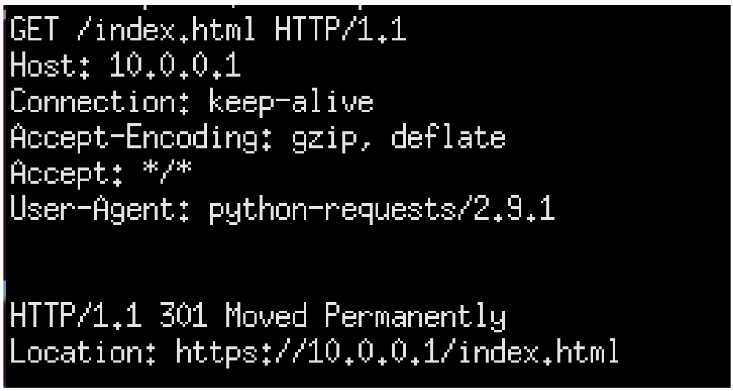
\includegraphics[width=0.35\textwidth]{result1.png}}
    \subfigure{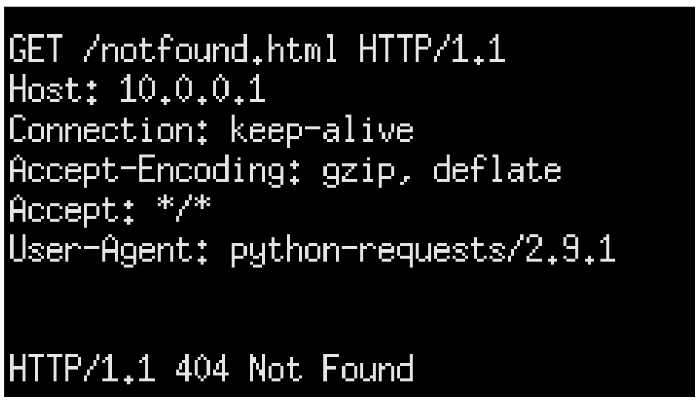
\includegraphics[width=0.35\textwidth]{result2.png}}
    \subfigure{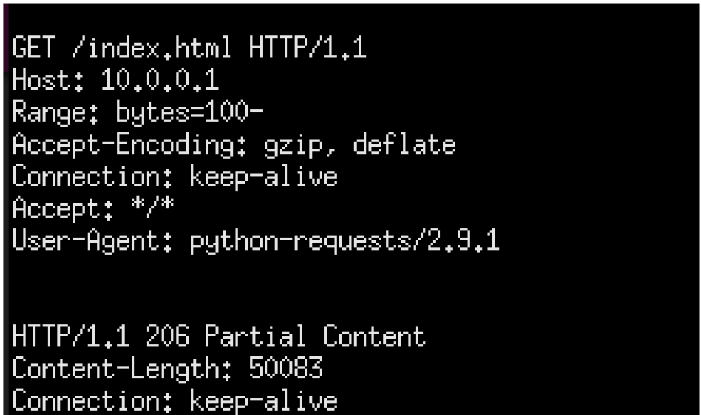
\includegraphics[width=0.35\textwidth]{result3.png}}
    \subfigure{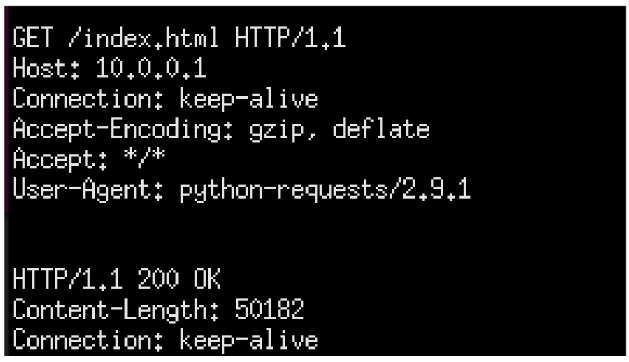
\includegraphics[width=0.35\textwidth]{result4.png}}
    \caption{测试程序结果}
\end{figure}

测试程序运行正常,没有出现AssertionError或其他错误,说明程序实现正确。

\section{实验总结}

本次实验实现了一个简单的HTTP服务器,支持GET方法,解析请求报文,返回相应应答及内容。通过实验,我学会了使用socket编程,实现HTTP服务器,了解了HTTP协议的基本内容,加深了对网络编程的理解。我在本次实验中所学到的知识也基本都是之前从未了解到的,对我来说是一次很好的学习机会。
\end{document}
